\chapter{Krav}
Til projektet er der opstillet to krav, som er formuleret i projektoplægget. Det er et krav at disse funktioner implementeres i produktet. Kravene lyder på at er skal udvikles et system, som kan tilsluttes et væskefyldt kateter samt vise en blodtrykskurve på en computerskærm. Mere detaljeret vil det sige at systemet skal indeholde to elementer. Først et elektronisk kredsløb, som forstærker signalet fra tryktransduceren og filtrerer det med et indbygget analogt filter. Derefter et program til at vise blodtrykket, som funktion af tiden.

Yderligere skal dette program opfylde kravene:
\begin{itemize}
\item Programmeres i C\#
\item Kunne kalibrere blodtrykssignalet og foretage en nulpunktsjustering
\item Vise blodtrykket kontinuert
\item Kunne lagre de målte data i en tekstfil eller en database
\item Kunne filtrere blodtrykket via et digitalt filter, denne funkton skal kunne slås til og fra
\end{itemize}

På baggrund af disse krav er der opstillet fem Use Cases, der tager højde for disse krav samt beskriver aktørens interaktion med systemet. Disse Use Cases benyttes som kravspecifikation, der har til formål at specificere, hvilke krav der stilles til projektet. Udover ovennævnte krav vil vi også arbejde hen imod at systemet skal afbillede puls, det systoliske blodtryk og det diastoliske blodtryk med tal. Derudover også at systemet alarmerer hvis blodtrykket overstiger indbyggede grænseværdier.
Kravene opstilles ud fra kundens ønsker samt leverandørens mulighed for realisering. Systemet består af en computer med programkode, en NI-DAQmx, en transducer og hardware printplade med et filter og en forstærker. Den fulde beskrivelse af hver enkelt Use Cases (fully dressed Use Cases) findes i dokumentationen. 

\begin{figure}[htb]
	\centering
	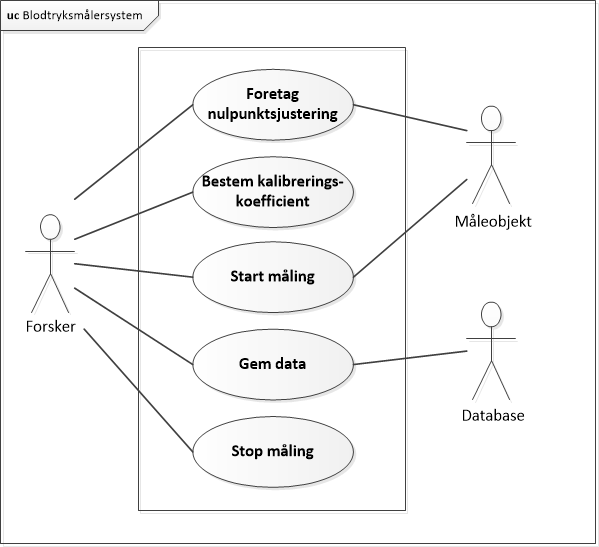
\includegraphics[width=0.6\textwidth]{Figurer/UseCasediagram}
	\caption{Use Case diagram}
	%\label{fig:Use Case diagrammet for blodtrykssystemet}
\end{figure}

\subsubsection{Aktørbeskrivelse}
Use Case diagrammet viser de tre aktører: Forsker, Database og Transducer. Herunder er der en detaljeret beskrivelse af hver aktør.

\textbf{Forsker} er en primær aktør. Det er denne aktør, som foretager blodtryksmålingen. Målingerne for blodtrykssignalet vises på displayet, som forskeren har tilgang til. 

\textbf{Transducer} er en sekundær aktør. Transduceren har til formål at modtage blodtrykssignalet fra måleobjektetet, som kan bestå af In Vitro, patient eller anden, som kan skabe en blodtrykssignal. 

\textbf{Database} er en sekundær aktør. Denne aktør er en database, hvori det ufiltrerede blodtrykssignal gemmes. Ligeledes gemmes det indtastede forsøgsnavn og det autogenerede nummer.

\subsubsection{Use Case beskrivelse}
Use Case diagrammet viser ligeledes de fem Use Cases, der er for systemet: Foretag nulpunktsjustering, Foretag kalibrering, Start Måling, Gem data, Afslut måling. Disse Use Cases beskriver interaktionen mellem aktørerne og systemet. Herunder er der en kort beskrivelse formålet med hver Use Case.

\textbf{UC1: Foretag nulpunktsjustering}
Forskeren tager stilling til om en nulpunktsjustering ønskes foretaget. Hvis nej, går systemet videre til næste Use Case. Hvis ja, påbegynder systemet en nulpunktsjustering, hvor en offset-værdi ud fra et kendt signal bestemmes. Denne offset-værdi justeres så ind, så en offset-værdi på nul indstillet. Således er en nulpunktsjustering foretaget.

\textbf{UC2: Foretag kalibrering}
Forskeren tager stilling til om en kalibrering ønskes foretaget. Hvis nej, går systemet videre til næste Use Case. Hvis ja, foretages en kalibrering. Det kræver at forskeren åbner for ventilen på transduceren, der er placeret på måleobjektet. Herefter modtager systemet så en værdi for det atmosfæriske tryk. Denne værdi korrigeres af en algoritme i systemet. Dermed er en kalibrering foretaget.  

\textbf{UC3: Start måling}
Det kræves at måleobjekt, hvor på blodtrykssignal ønskes fra, er tilsluttet. Derfor tilslutter forskeren transduceren til måleobjektet. Derpå kan målingen startes ved at forskeren trykker på knappen START MÅLING. Herefter indhenter systemet blodtrykssignalet, som bliver udskrevet på display. Værdier for puls, systolisk- og diastolisk blodtryk udskrives ligeledes på display. 

\textbf{UC4: Gem data}
Det er muligt for forskeren at gemme det indhentet ufiltrerede blodtrykssignal, inden for en periode valgt af forskeren. Dette gøres ved, at forskeren trykker på knappen GEM. Systemet vil herefter begynde at sende signaldata ind i databasen, hvor dataene gemmes. Dette vil systemet blive ved med at udføre indtil forskeren trykker på knappen GEM igen eller knappen AFSLUT.  

\textbf{UC5: Afslut måling}
Det er muligt for forskeren at lukke systemet ned. Dette gøres ved, at forskeren trykker på knappen AFSLUT. Systemet vil herefter afslutte igangværende processer og lukke ned.

\subsubsection{Ikke-funktionelle krav beskrivelse}
Ikke-funktionelle krav er struktureret efter (F)URPS+, hvor krav til systemets funktionalitet, brugervenlighed, pålidelighed, præsentation samt vedligehold er beskrevet. Disse krav er primært software-krav. Der opstilles bl.a. et krav om en maksimal tid, der må gå fra, at der er trykket på en knap, til at systemet reagerer. Når der er trykket på en knap, skal systemet foretage den ønskede proces, hvilket eksempelvis er, at ved tryk på GEM-knappen at sende det ufiltrerede blodtrykssignal til databasen, hvor signaldata bliver gemt. Ligeledes er opbygning af display også en del af de ikke-funktionelle krav.